\documentclass[tikz,border=8pt]{standalone}
\usepackage{tikz}
\usetikzlibrary{arrows.meta,positioning,calc,backgrounds,fit,shapes.geometric}
\usepackage[scaled=0.92]{helvet}
\renewcommand{\familydefault}{\sfdefault}
\usepackage{amsmath,amssymb}
\definecolor{ink}{HTML}{262624}
\definecolor{mute}{HTML}{8A8984}
\definecolor{line}{HTML}{BDBBB5}
\definecolor{acc}{HTML}{2A78D6}
\definecolor{accbg}{HTML}{F1F6FD}
\tikzset{
  >={Latex[length=2.2mm]},
  every node/.style={text=ink},
  b/.style={draw=line, fill=white, rounded corners=2pt, align=center, inner sep=6pt,
            minimum height=10mm, text width=#1, font=\small},
  b/.default=40mm,
  a/.style={b=#1, draw=acc, fill=accbg},
  a/.default=40mm,
  t/.style={font=\footnotesize, text=mute, align=center},
  e/.style={->, draw=mute, line width=0.6pt},
  ea/.style={->, draw=acc, line width=0.9pt},
  eh/.style={->, draw=acc, line width=0.9pt, dash pattern=on 3pt off 2pt},
}

\begin{document}
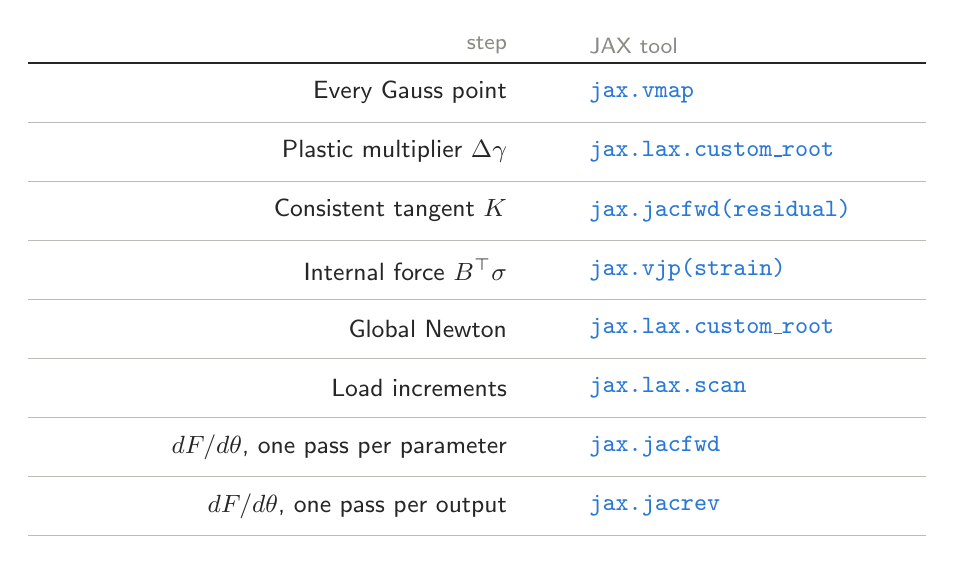
\begin{tikzpicture}
\newcommand{\row}[3]{%
  \node[anchor=east, font=\small] at (0,-0.75*#1) {#2};
  \node[anchor=west, font=\ttfamily\small, text=acc] at (0.8,-0.75*#1) {jax.#3};
  \draw[line, line width=0.4pt] (-6.2,-0.75*#1-0.375) -- (5.2,-0.75*#1-0.375);}
\row{0}{Every Gauss point}{vmap}
\row{1}{Plastic multiplier $\Delta\gamma$}{lax.custom\_root}
\row{2}{Consistent tangent $K$}{jacfwd(residual)}
\row{3}{Internal force $B^{\top}\sigma$}{vjp(strain)}
\row{4}{Global Newton}{lax.custom\_root}
\row{5}{Load increments}{lax.scan}
\row{6}{$dF/d\theta$, one pass per parameter}{jacfwd}
\row{7}{$dF/d\theta$, one pass per output}{jacrev}
\node[anchor=east, t] at (0,0.6) {step};
\node[anchor=west, t] at (0.8,0.6) {JAX tool};
\draw[ink, line width=0.6pt] (-6.2,0.375) -- (5.2,0.375);
\end{tikzpicture}
\end{document}
